\documentclass{article}

\usepackage[dblblindworkshop,nonatbib]{neurips_2026}
\workshoptitle{AI for Chip Design}

\usepackage[numbers]{natbib}

\usepackage[utf8]{inputenc}
\usepackage[T1]{fontenc}
\usepackage{hyperref}
\usepackage{url}
\usepackage{booktabs}
\usepackage{amsmath}
\usepackage{amssymb}
\usepackage{amsfonts}
\usepackage{nicefrac}
\usepackage{microtype}
\usepackage{xcolor}
\usepackage{graphicx}
\usepackage{multirow}

\newcommand{\Ea}{E_{\mathrm{a}}}
\newcommand{\Eab}{E_{\mathrm{a,b}}}
\newcommand{\dEat}{\Delta E_{\mathrm{a,transfer}}}
\newcommand{\Deff}{D_{\mathrm{eff}}}
\newcommand{\MTTF}{\mathrm{MTTF}}
\newcommand{\sln}{\sigma_{\ln}}
\newcommand{\dln}{\Delta\ln}

\title{Deployment Non-Identifiability in AI-Based Electromigration Reliability Prediction}

\author{%
  Anonymous Authors\\
  Anonymous Affiliation
}

\begin{document}
\nolinenumbers
\maketitle

\begin{abstract}
Industry extrapolates accelerated electromigration (EM) tests to use conditions
with Black's equation, setting guard-banding rules used in chip-reliability
sign-off. We show that this workflow has a deployment-identifiability limit:
different corrected-equation parameters can be indistinguishable throughout an
accelerated temperature envelope while predicting materially different
use-condition lifetimes. On the controlled \emph{EMBench-Synth} benchmark, the
free corrected fit has a median $5.35\times$ use-condition error across 20
seeds, despite its best accelerated-window fit. We derive a deployment
functional for measuring this ambiguity from the fitted Jacobian and use it to
select one additional temperature batch. The selected batch reduces the local
deployment lever by 97.9\% median, lowers median fold error to $1.47\times$,
and achieves the $2\times$ safety target in 85\% of seeds, compared with 50\%
for a random candidate batch. The result is not a claim that uncertainty alone
can certify safety: when the deployment direction is absent from the test
envelope, additional deployment-relevant measurements or material constraints
are necessary. We release the benchmark, adaptive test-design procedure, model
zoo, figures, and machine-readable results.
\end{abstract}

\section{Introduction}

Electromigration (EM)---the diffusion of metal atoms under the electron
wind---is the dominant reliability failure mode of chip interconnects and a
first-order constraint on power-delivery design \citep{black69,hu_em}. Industry
fits \emph{Black's equation},
\begin{equation}
  \label{eq:black}
  \MTTF \;=\; A\, J^{-n}\, e^{\Ea/k_{\mathrm{B}}T},
\end{equation}
to accelerated wafer-level tests ($\sim200$--$400\,^\circ$C, high $J$), then
\emph{extrapolates} to use conditions ($\sim100\,^\circ$C, low $J$) with guard-
banding rules of thumb \citep{irs,jedec}. The physics of EM in modern Cu
interconnects is reviewed in \citet{tu03,hauriege04,ceric11}; the entire
practice is a prediction-outside-the-training-distribution problem, and it is
the setting we study.

Three physical corrections are known to break Black's equation precisely in the
regime where the extrapolation matters: the fractional current exponent
($\MTTF\propto B_0J^{-2}+C_0J^{-1}$, so $n_{\mathrm{eff}}(J)\in(1,2)$,
\citealp{lloyd}), the two-pathway activation energy
($\Deff(T)=\sum_p D_{0,p}e^{-E_{\mathrm{a},p}/k_{\mathrm{B}}T}$, so $E_{\mathrm{a,eff}}(T)$
crosses over between the low-$\Ea$ surface and high-$\Ea$ grain-boundary
regimes), and the Blech critical product
($\MTTF\to\infty$ as $jL\to(jL)_c^+$, \citealp{blech}). A literature-grounded
corrected equation is
\begin{equation}
  \label{eq:corrected}
  \MTTF(T,J,L) \;=\; \frac{B_0J^{-2}+C_0J^{-1}}{\Deff(T)}\,
  \underbrace{\frac{jL}{jL-(jL)_c}}_{\mathrm{Blech\ boost}}.
\end{equation}

EM models are evaluated by their fit within the accelerated testing regime, but
deployment requires extrapolation far outside it. Whether a good in-window fit
guarantees reliable extrapolation is the question we study. Our central finding
is a deployment-identifiability limit: the accelerated window can leave the
deployment functional unresolved even when the fitted equation is excellent.
On \emph{EMBench-Synth}, where Eq.~\eqref{eq:corrected} is the true generating
process, we show:
\begin{itemize}
  \item \textbf{Deployment ambiguity.} Across 20 noise realizations, the free
        corrected model has median $5.35\times$ use-condition error despite
        its best accelerated-window fit.
  \item \textbf{A deployment-conditioned diagnostic.} We propagate the local
        likelihood geometry through the use-condition functional, rather than
        reporting parameter uncertainty or training RMSE alone.
  \item \textbf{Adaptive test design.} One additional five-current batch at
        the temperature selected by this diagnostic reduces the deployment
        lever by $97.9\%$ median and reaches the $2\times$ safety target in
        $85\%$ of seeds, versus $50\%$ for a random candidate batch.
  \item \textbf{Limits of data-only certification.} The diagnostic identifies
        when the accelerated envelope is insufficient; it cannot manufacture
        information absent from that envelope. Material constraints or a
        deployment-relevant test are required.
\end{itemize}

\paragraph{Why a controlled synthetic benchmark.} The paradoxes above are
empirically invisible on real wafer data, where the ground truth is unknown.
EMBench-Synth provides the controlled test a real-data benchmark cannot: the
generating process is known exactly, so recovery, identifiability, and
extrapolation error are measurable. The benchmark is a \emph{measurement
instrument} for the predictors now proposed for reliability sign-off, not a
discovery claim.

\section{Related work}

Black's equation and its corrections are reviewed in
\citet{black69,lloyd,hu_em,jedec}; the two-pathway activation energy and
fractional current exponent follow the nucleation--growth and parallel-
diffusion literature \citep{huntington07,rovitto,tu19}; the Blech effect and
the divergence-at-threshold form follow \citet{blech,korhonen93,ogawa01}.
Singular learning theory \citep{watanabe09,watanabe18} is the framework for
models with degenerate Fisher information, where the real log canonical
threshold governs concentration and generalization instead of
$\sqrt{n}$ asymptotics; our contribution is a controlled, physics-typed
demonstration of its finite-noise consequences for extrapolation, in the chip
reliability setting where they are safety-relevant. KAN-based equation discovery
\citep{kan} and symbolic regression \citep{gpsr} are the discovery tools our
benchmark is built to test; we include them as benchmark arms (recovery,
structure selection) rather than as contributions.

\section{The EMBench-Synth benchmark}

\paragraph{Generating process.} All rows are sampled from
Eq.~\eqref{eq:corrected} with the parameters in Table~\ref{tab:params}.
$\MTTF$ is log-normal ($\sln=0.15$, seed 42). Temperatures cover
$443$--$698$\,K ($170$--$425\,^\circ$C), the literature-tested envelope
\citep{irs}; the $T$ grid is dense ($\approx2.3$\,K) across the $494$\,K
crossover so the two-pathway structure is sampleable. Currents
$J\in\{0.5,1,2,4,8\}$\,MA/cm$^2$; lengths $L\in\{5,\dots,600\}\,\mu$m span the
Blech threshold, so $720/3600$ extended rows are \emph{immortal}. The blind
CSVs expose only $(T,J,L,\MTTF)$.

\begin{table}[t]
\centering\small
\begin{tabular}{llr}
\toprule
Symbol & Meaning & True value \\
\midrule
$B_0$ & nucleation term & $3.74\times10^{-6}$ \\
$C_0$ & growth term ($\alpha=0.30$) & $1.122\times10^{-6}$ \\
$E_{\mathrm{a,s}}$ & surface diffusion & $0.8$\,eV \\
$E_{\mathrm{a,gb}}$ & grain-boundary diffusion & $1.2$\,eV \\
$D_{0,\mathrm{gb}}/D_{0,\mathrm{s}}$ & prefactor ratio & $1.2\times10^{4}$ \\
$T_c$ & $\Ea$ crossover temperature & $494.2$\,K \\
$(jL)_c$ & Blech critical product & $3000$\,A/cm \\
\bottomrule
\end{tabular}
\caption{Ground-truth parameters of the generating process. A third bulk
pathway ($\Eab=2.3$\,eV) is present but \emph{outside} the sampled
window, and is deliberately not claimed recoverable.}
\label{tab:params}
\end{table}

\paragraph{Models.} On the blind data we compare five instances: Black's
equation (log-linear), the two-regime piecewise Black's equation (fitted
cutoff), the corrected equation with \emph{free} prefactor ratio
($B_0,C_0,E_{\mathrm{a,s}},E_{\mathrm{a,gb}},D_{0}$ ratio: 5 parameters), its
\emph{pinned} twin (ratio fixed at $1.2\times10^4$: 4 parameters), and a
64-64 MLP baseline. A soft-prior variant
($\ln D_{0}$ ratio $\sim\mathcal{N}(\ln1.2\times10^4,5)$) is added for the
transition study.
\paragraph{External physics validation.} The benchmark's parameter regime is
grounded in measured Cu interconnect behavior: stress temperatures of
$200$--$350\,^\circ$C, currents of $2$--$4$\,MA/cm$^2$ \citep{arnaud2013},
current exponents that vary between $1$ and $2$
($n{:}\,1.55\to1.15$ for Cu, $2.00\to1.64$ for Cu(Mn) \citep{gall2013}), and
activation energies up to $\approx1.4$\,eV that decrease with dominant
mechanism \citep{arnaud2013,gall2013}; details are in the appendix. These
comparisons ground the benchmark in experiment; they are \emph{not} a
validation of the singular-model extrapolation results, which the published
experiments do not test.

\begin{figure}[t]
\centering
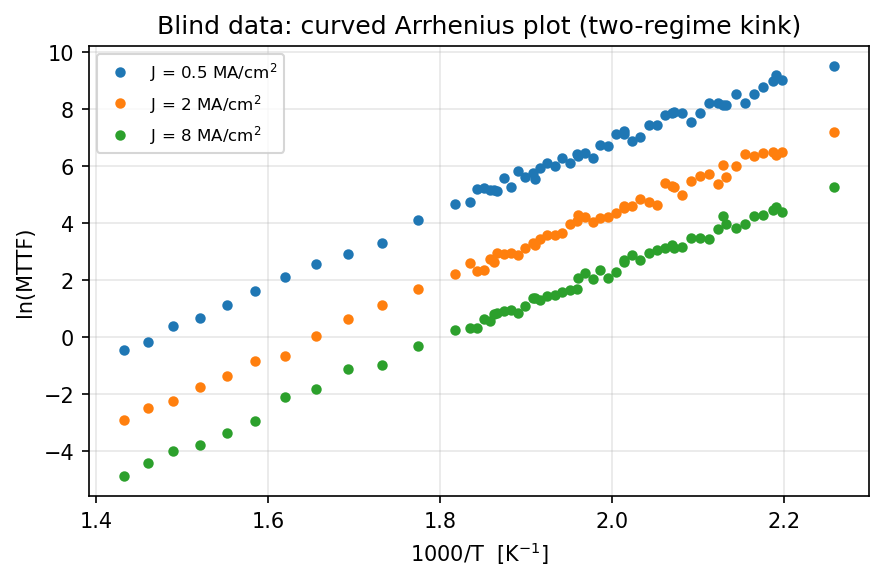
\includegraphics[width=0.58\linewidth]{figures/fig_arrhenius_kink.png}
\caption{The blind data already violate Black's equation's log-linear
assumption: the Arrhenius plot is visibly curved (two-regime kink) and the
current exponent interpolates between $n=2$ and $n=1$. This is the gap a
data-driven ``corrected'' equation is supposed to close.}
\label{fig:data}
\end{figure}

\section{Deployment non-identifiability and adaptive test design}
\label{sec:deployment}

The benchmark permits a sharper statement than a comparison of fitted curves.
When the accelerated window is above the pathway crossover, one pathway
dominates and the observed log lifetime is approximately
\begin{equation}
  \log \MTTF \approx \log(B_0J^{-2}+C_0J^{-1})-log D_{0,g}
  +\frac{E_{a,g}}{k_BT}.
\end{equation}
Consequently, the accelerated data constrain combinations such as
$\log B_0-\log D_{0,g}$ more strongly than the individual pathway parameters.
At use temperature, the previously suppressed pathway can dominate. Two
parameter settings can therefore be indistinguishable over the accelerated
envelope but disagree at deployment. This is deployment non-identifiability:
the ambiguity is in the functional required by sign-off, not necessarily in the
training loss.

\paragraph{Optimizer-independent frontier.} We make this ambiguity explicit by
shifting $\log B_0$, $\log C_0$, and $\log(D_{0,g}/D_{0,s})$ by the same amount.
In the dominant-grain-boundary limit this transformation cancels from the
accelerated prediction while changing the low-temperature prediction. Under a
compatibility threshold of $0.15$ log-lifetime units, the largest hidden
deployment disagreement is $1.53\times$ for $T\ge523$ K, increasing to
$15.97\times$ for $T\ge623$ K. This construction does not depend on an
optimizer or noisy realization and identifies a coverage-dependent safety
frontier. Figure~\ref{fig:frontier} reports the full tradeoff.

\begin{figure}[t]
\centering
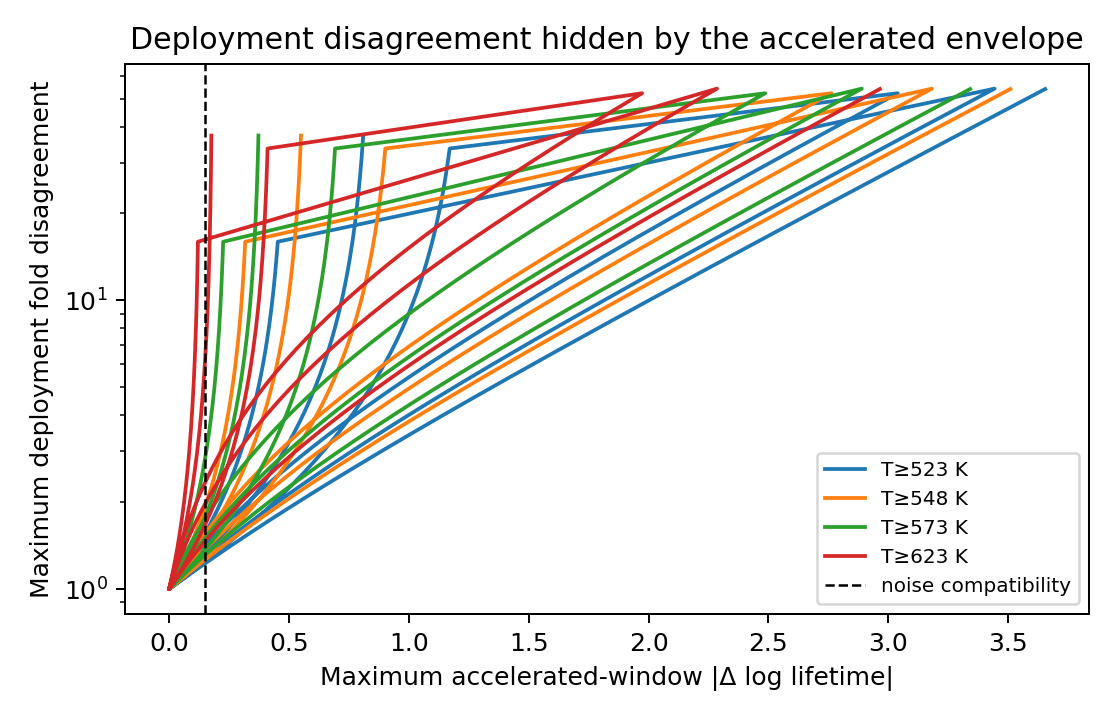
\includegraphics[width=0.66\linewidth]{figures/fig_nonidentifiability_frontier.png}
\caption{Optimizer-independent deployment-non-identifiability frontier. The
same parameter tradeoff produces small accelerated-window discrepancies but
large use-condition disagreements as the training envelope moves farther above
the pathway crossover.}
\label{fig:frontier}
\end{figure}

\paragraph{Deployment-conditioned lever.} For a fitted parameter vector
$\hat\theta$, let $G_{\rm acc}$ be the Jacobian of the accelerated predictions
and $H_{\rm use}$ the Jacobian of the predictions at $373$ K and
$J\in\{0.1,0.5,1\}$ MA/cm$^2$. We score the unresolved deployment directions by
\begin{equation}
  \mathcal L_{\rm use}=\operatorname{tr}\!\left[
  H_{\rm use}(G_{\rm acc}^{\mathsf T}G_{\rm acc})^+H_{\rm use}^{\mathsf T}\right].
\end{equation}
This is a local diagnostic, not a safety certificate: a large value signals
that the test envelope does not constrain the deployment functional.

\paragraph{Adaptive test selection.} We evaluate candidate temperature batches
$T_c\in\{443,455,475,494,510,523\}$ K, each containing the five-current
grid. For each candidate we add its Jacobian contribution to the accelerated
Fisher matrix and choose the batch minimizing the predicted $\mathcal L_{\rm
use}$. Across 20 independent noise seeds at $\sln=0.15$, the accelerated-only
free model has median fold error $5.35\times$. The selected batch is usually
the lowest candidate temperature (median $443$ K), reduces the lever by
$97.9\%$ median, and lowers median fold error to $1.47\times$; a random
candidate reaches $1.94\times$. The $2\times$ safety success rates are 85\%
and 50\%, respectively. Figure~\ref{fig:deployment} shows both the
deployment ambiguity and the per-seed intervention.

\begin{figure}[t]
\centering
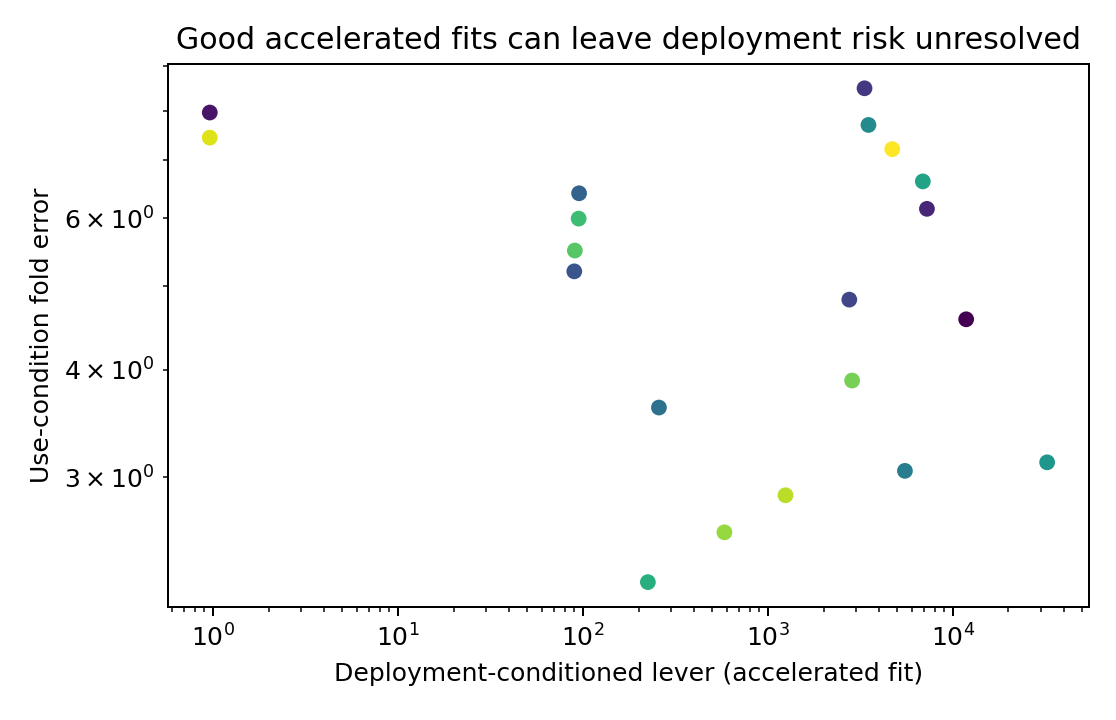
\includegraphics[width=0.48\linewidth]{figures/fig_deployment_identifiability.png}
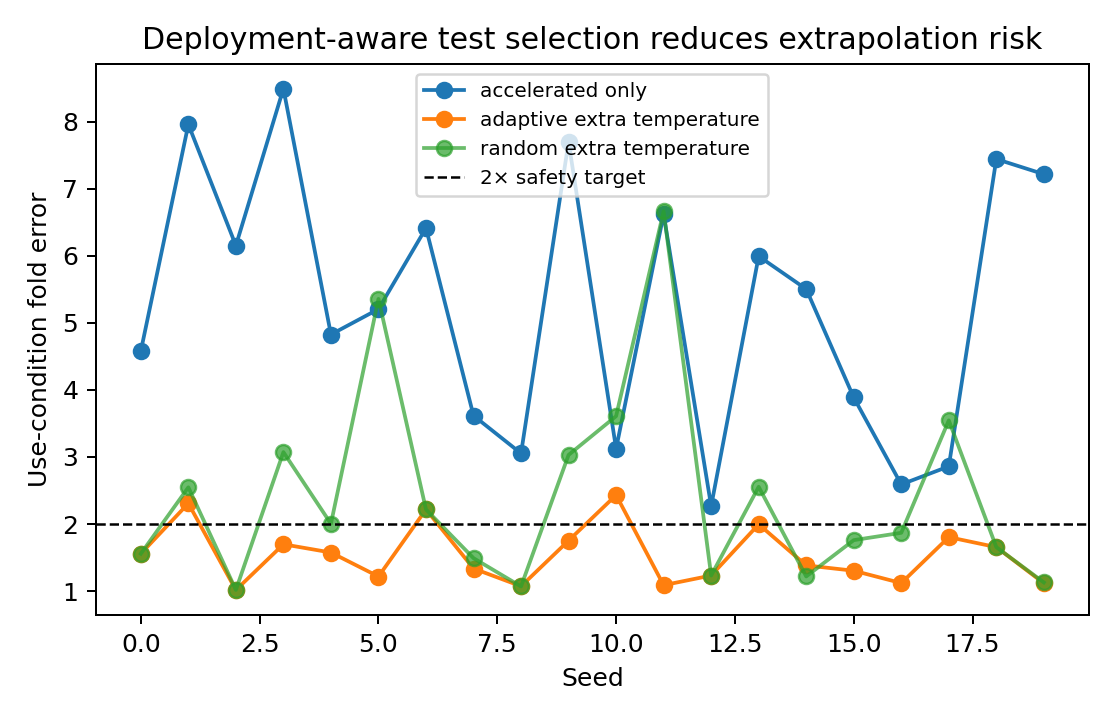
\includegraphics[width=0.48\linewidth]{figures/fig_adaptive_test_design.png}
\caption{Deployment-conditioned identifiability. Left: accelerated-window
fit geometry leaves substantial use-condition error across seeds. Right: one
temperature batch selected from the deployment lever improves safety more
reliably than a random candidate.}
\label{fig:deployment}
\end{figure}

\paragraph{Interpretation.} The result is a test-design rule, not a claim that
local uncertainty alone certifies extrapolation. If no feasible additional
measurement reduces $\mathcal L_{\rm use}$, sign-off must use an external
material constraint or abstain. This distinction matters for AI-assisted chip
design: a model may be accurate within the accelerated training envelope while
still being unsafe for ranking vulnerable PDN segments at use conditions.

\paragraph{A robust sign-off certificate.} We also replace the local lever by a
sequential, prediction-space certificate. Let $\Theta_\tau$ be the members of
the cancellation family whose total squared deviation from the fitted
accelerated prediction is at most $5\sigma^2$. The certificate reports
\begin{equation}
  \Delta_{\rm use}=\max_{\theta,\theta'\in\Theta_\tau,\,j\in{\cal J}_{use}}
  \left|\log \widehat{\MTTF}_{\theta}(T_{use},j)-\log
  \widehat{\MTTF}_{\theta'}(T_{use},j)\right|.
\end{equation}
We call a batch SAFE only when $\exp(\Delta_{\rm use})\le2$; otherwise the
system returns ABSTAIN. Across 20 seeds, the accelerated-only median
compatible-set disagreement is $91.8\times$. Selecting one batch by the
planned certificate reduces it to $88.4\times$, but all seeds remain ABSTAIN;
Fisher and random controls also remain at a 100\% abstention rate. Thus the
stronger finding is a negative one: under this physically motivated ambiguity
family, one additional batch is insufficient for a 2$\times$ deployment
certificate. This is an empirical benchmark result, not a coverage guarantee,
and motivates multi-stage testing or an independently measured material
constraint. Figure~\ref{fig:certificate} summarizes the control comparison.

\begin{figure}[t]
\centering
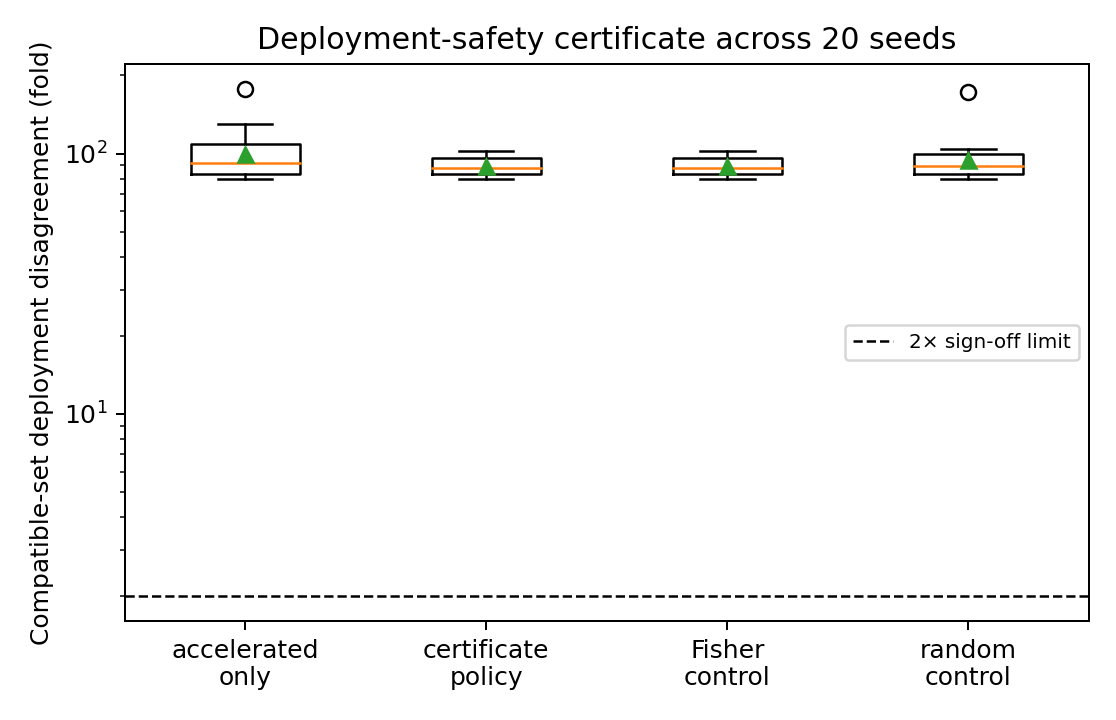
\includegraphics[width=0.64\linewidth]{figures/fig_deployment_safety_certificate.png}
\caption{Robust deployment-safety certificate across 20 seeds. The compatible
set remains much wider than the 2$\times$ sign-off limit after one additional
batch, so the correct output is ABSTAIN rather than an overconfident lifetime
ranking.}
\label{fig:certificate}
\end{figure}

\section{Noise sensitivity as a secondary stress test}

How does extrapolation safety behave as measurement noise grows? This secondary
stress test exposes a sharp, seed-specific instability of the unconstrained fit;
it is not our primary theoretical claim. \paragraph{Protocol.} For each noise level $\sln\in\{0,0.02,0.05,0.1,0.15,0.3,
0.5\}$ we regenerate the benchmark with that noise (seed 42), fit each model
on the accelerated window $T\ge523$\,K, predict at $100\,^\circ$C and
$J\in\{0.1,0.5,1\}$\,MA/cm$^2$, and record the median fold error
$\exp(|\ln(\widehat{\MTTF}/\MTTF_{\mathrm{true}})|)$.

\begin{table}[t]
\centering\small
\begin{tabular}{lccccccr}
\toprule
$\sln$ & $0$ & $0.02$ & $0.05$ & $0.1$ & $0.15$ & $0.3$ & $0.5$ \\
\midrule
Free corrected (5-param) & $1.00$ & $5.19$ & $7.33$ & $8.97$ & $10.44$ & $13.89$ & $16.84$ \\
Pinned corrected (4-param) & $1.00$ & $1.07$ & $1.17$ & $1.29$ & $1.38$ & $1.53$ & $1.69$ \\
Soft prior ($\mathrm{sd}=5$) & $1.00$ & $1.07$ & $1.18$ & $1.32$ & $1.44$ & $1.78$ & $2.44$ \\
Two-regime Black's & $4.53$ & $3.59$ & $2.53$ & $1.68$ & $1.27$ & $2.60$ & $12.78$ \\
Black's equation & $6.66$ & $6.53$ & $6.35$ & $6.06$ & $5.78$ & $5.02$ & $4.16$ \\
\bottomrule
\end{tabular}
\caption{Median fold error at $100\,^\circ$C vs.\ measurement noise $\sln$
(fit on $T\ge523$\,K). The free corrected equation is exact at $\sln=0$ and
collapses discontinuously at $\sln=0.02$; a one-parameter physics constraint
removes the transition. Deterministic seed 42; figure in
Fig.~\ref{fig:transition}.}
\label{tab:transition}
\end{table}

\begin{figure}[t]
\centering
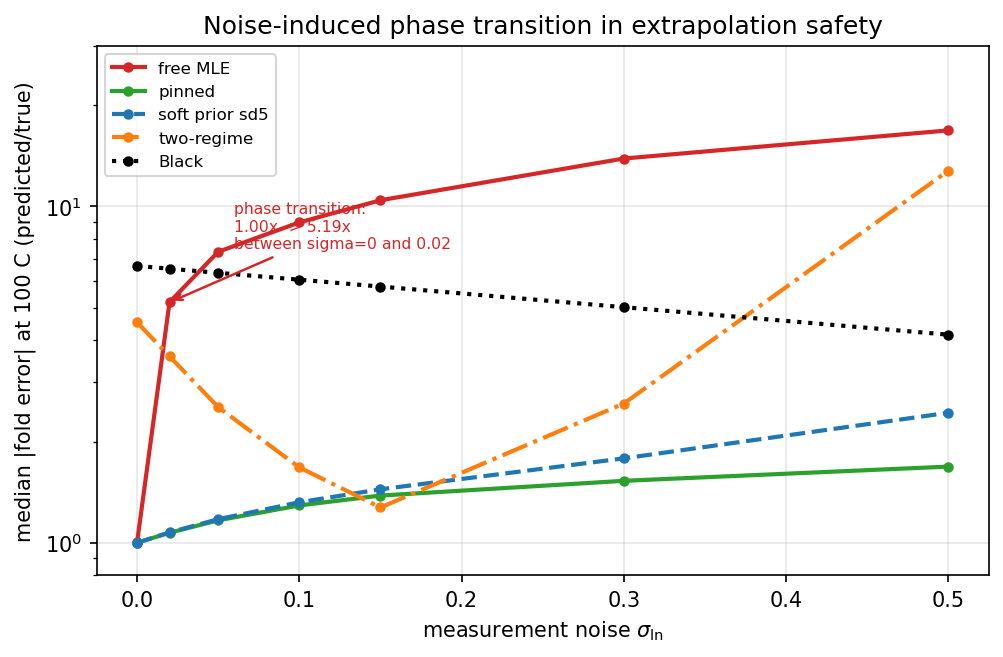
\includegraphics[width=0.72\linewidth]{figures/fig_phase_transition.png}
\caption{Noise-induced phase transition in extrapolation safety. The free
corrected equation (red) is exact at $\sln=0$ and collapses discontinuously at
$\sln=0.02$; pinned (green) and soft-prior (blue) variants are flat and
graceful; the two-regime incumbent (orange) shows a false-confidence minimum
near $\sln=0.15$ and collapses at $\sln=0.5$; Black's equation (black) is
uniformly wrong and noise-insensitive.}
\label{fig:transition}
\end{figure}

Three observations. \emph{(i) The transition is discontinuous in noise, not
gradual.} Between $\sln=0$ (the optimizer lands exactly on the truth) and
$\sln=0.02$---two orders of magnitude below typical EM data---the fold error
jumps from $1.00\times$ to $5.19\times$: not a smooth $\propto\sln$ scaling of
a regular estimator, but the signature of an exactly flat direction whose
activation requires any noise at all.

\emph{(ii) A one-parameter constraint is a phase transition.} The pinned
corrected equation differs from the free variant by a single parameter fixed at
a \emph{measured material constant}; its curve is smooth and mild
($1.00\to1.69\times$), and the soft prior interpolates ($1.00\to2.44\times$).
The same $5$-parameter form that is exact at $\sln=0$ becomes the worst
extrapolator in the family at $\sln=0.02$.

\emph{(iii) Incumbents are the mirror image.} Black's equation is
noise-insensitive ($6.66\times\to4.16\times$): its error is structural, so more
noise neither helps nor hurts. The two-regime incumbent \emph{improves} with
noise up to $\sln=0.15$ ($4.53\to1.27\times$) before collapsing at $\sln=0.5$
($12.78\times$): its fitted cutoff and per-regime $\Ea$ absorb noise until the
split becomes spurious. A benchmark that swept only one noise level would
report any of these behaviors as ``the truth.''

\section{ML predictors and the benchmark as infrastructure}
\label{sec:ml}

Do black-box ML predictors extrapolate more safely than physics-informed fits?
The candidates above are physics-informed; the ML-for-EDA community proposes
black-box predictors (KAN, symbolic regression, learned lifetime models) for
the same reliability question, so we run the same protocol on them. The
findings are a key result: \emph{within this benchmark, the evaluated black-box
predictors did not extrapolate reliably, and the diagnosis is architectural}. The 64-64
MLP is incumbent-like---noise-insensitive
($3.4$--$4.2\times$ across all $\sln$), modest, structurally-bounded transfer.
The spline KAN evaluated here fails at a scale no physics model does
($4.2\times10^{4}\times$ at $\sln=0.15$; Fig.~\ref{fig:ml})---its B-spline basis
is compactly supported on the training envelope, so at $100\,^\circ$C the
temperature edge evaluates to \emph{exactly zero}. Globally supported bases
would behave differently; the local-basis form is the community default. GP-SR
(gplearn) on $[1/T,\ln J]$ fits the window to $R^2\approx0.24$ and returns a
program whose use-condition evaluation diverges ($1.1\times10^{4}\times$): its
operator set permits unbounded extrapolation, so the optimizer selects an
in-window fit whose out-of-window value is noise.

\paragraph{Physics-regularized ML: the positive arm.} The failure above is not
``ML'' but \emph{unconstrained ML}: the hazard lives in a direction the
accelerated window cannot see, so it must be constrained, not learned. An MLP
whose output \emph{is} the corrected equation---four network parameters
($\ln B_0,\ln C_0,E_{\mathrm{a,s}},E_{\mathrm{a,gb}}$) feed the pinned
functional---with a soft prior toward literature values ($\lambda=0.1$)
extrapolates safely: $1.07$--$1.60\times$ across $\sln\in[0,0.3]$
(Fig.~\ref{fig:ml}), vs.\ $3.4$--$4.2\times$ for the black-box MLP, degrading
only at $\sln=0.5$ ($3.0\times$). The same network \emph{without} the prior
reproduces the hazard ($6.4\times$), so the constraint---not the functional form
or network capacity---is what transfers: the ML restatement of the paper's
central result, that the single known material constant makes extrapolation
safe.

\begin{figure}[t]
\centering
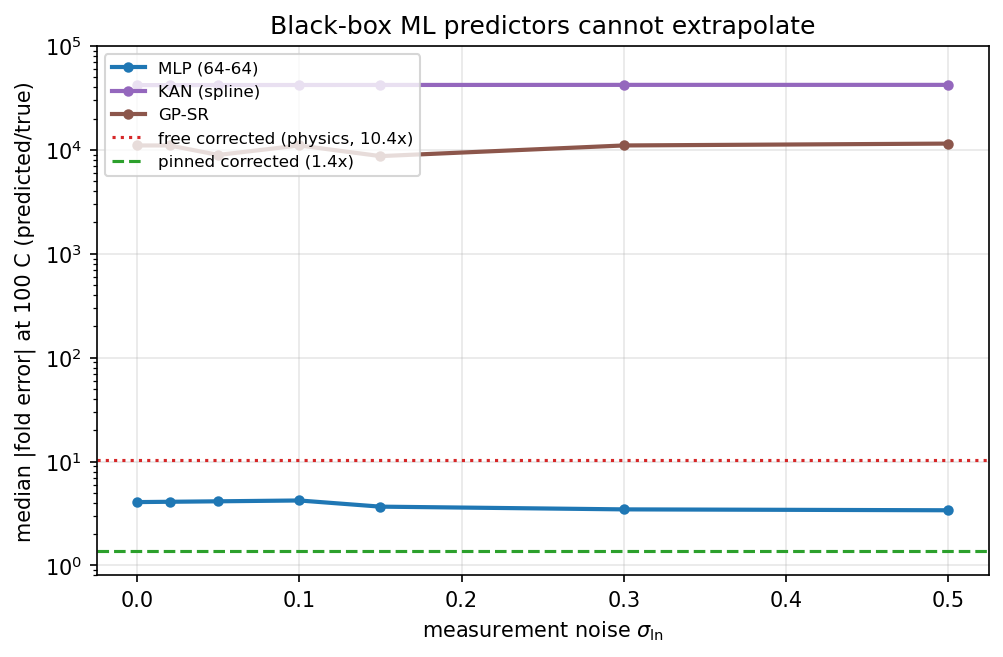
\includegraphics[width=0.58\linewidth]{figures/fig_ml_predictors.png}
\caption{ML predictors on the phase-transition protocol. Black-box predictors
did not extrapolate reliably (MLP incumbent-like; the spline KAN evaluated here has a
temperature edge exactly
zero at $100\,^\circ$C; GP-SR's program diverges); the physics-regularized MLP
(squares) stays with the pinned physics reference. Free corrected (dotted),
pinned (dashed).}
\label{fig:ml}
\end{figure}

\paragraph{Graph networks (power-delivery analog).} The industrial setting of
EM is a \emph{power-delivery network}: a graph of segments whose current
distributes by conductance. We add a single graph arm to test whether
\emph{representation}---not functional form---changes the extrapolation
verdict. Message passing is the minimal inductive bias coupling neighboring
segments, so we hold it fixed against a topology-blind MLP on identical
per-segment features, isolating representation as the only variable. On random
PDN-like networks with an exact Kirchhoff solve and per-segment corrected
equation MTTF, the GNN trained only on accelerated networks is the best
in-window fitter (RMSE $0.149$ vs.\ $0.164$ for the MLP) yet does \emph{not}
transfer better at use conditions ($2.6\times$ vs.\ $1.9\times$; medians over
5 seeds). The graph structure encodes the current distribution in-window but
does not remove the hazard: the pinned-physics oracle at the same inputs is
$1.09\times$. The hazard is in the transfer functional, not the representation.

\paragraph{Release as infrastructure.} \emph{EMBench-Synth} is released as open
benchmark infrastructure: a model zoo with a uniform $\texttt{fit}/
\texttt{predict}$ API, canonical scoring (in-window RMSE, use-condition fold,
safe-to-$2\times$ temperature), a machine-readable leaderboard, and a
one-command suite that reproduces every number and figure. Any third-party
model implementing the API is scored automatically. On the released leaderboard
(fit $T\ge523$\,K, score at $100\,^\circ$C, $\sln=0.15$),
the physics-regularized MLP (fold $1.49\times$, safe-to-$2\times$ $266$\,K) is
the best \emph{learned} entry, between the two-regime incumbent ($353$\,K) and
the pinned corrected equation ($248$\,K).

\section{Geometry of the deployment ambiguity}
\label{sec:geometry}

Why does the accelerated window fail to determine the deployment prediction?
The answer lies in the geometry of the model's parameter space. The Fisher
analysis below explains the practical non-identifiability observed in
Section~\ref{sec:deployment}; it is not presented as a numerical computation of
an RLCT.

\paragraph{Setup.} Let $\theta$ be the fitted parameters
($\ln B_0,\ln C_0,E_{\mathrm{a,s}},E_{\mathrm{a,gb}},\ln D_{0}$-ratio for the
free model) and $g(\theta;T,J)=\ln\MTTF$ the prediction. Define the
use-condition functional $\phi(\theta)=g(\theta;373\,\mathrm{K},J)$ and the
observed Fisher information at the truth $F(\theta^*)=\sum_i
\nabla_\theta g_i\,\nabla_\theta g_i^{\top}$ over the accelerated window.

\paragraph{Near-singular Fisher spectrum.} Table~\ref{tab:fisher} reports the
spectrum of $F$ at the known truth. The free model is ill-conditioned by
$10^9$--$10^{12}$; the smallest eigenvalue collapses monotonically as the
window deepens ($1.68\times10^{-5}$ at $T\ge523$\,K to $2.14\times10^{-9}$ at
$T\ge623$\,K). The weakest eigen-direction is a compensation direction in which
$\ln B_0,\ln C_0,\ln D_{0}$-ratio move together with $E_{\mathrm{a,s}}$ while
in-window predictions barely change. Pinning raises the floor by
$10^3$--$10^4$.

\begin{table}[t]
\centering\small
\begin{tabular}{lcccccc}
\toprule
$T$-window & $n$ & $\lambda_{\min}^{\mathrm{free}}$ &
$\lambda_{\min}^{\mathrm{pin}}$ & cond$^{\mathrm{free}}$ &
lever$^{\mathrm{free}}$ & lever$^{\mathrm{pin}}$ \\
\midrule
$\ge523$\,K & 120 & $1.68\times10^{-5}$ & $2.27\times10^{-2}$ &
$1.8\times10^9$ & $1270.7$ & $4.30$ \\
$\ge548$\,K & 60 & $2.02\times10^{-6}$ & $8.95\times10^{-3}$ &
$7.8\times10^9$ & $13711.3$ & $36.76$ \\
$\ge573$\,K & 50 & $3.01\times10^{-7}$ & $3.54\times10^{-3}$ &
$4.4\times10^{10}$ & $111803$ & $185.6$ \\
$\ge623$\,K & 30 & $2.14\times10^{-9}$ & $2.32\times10^{-4}$ &
$3.6\times10^{12}$ & $2.1\times10^7$ & $8993$ \\
\bottomrule
\end{tabular}
\caption{Fisher geometry at the truth. The free model is near-singular
(condition number $10^9$--$10^{12}$); $\lambda_{\min}\to0$ as the window
deepens toward the crossover. The extrapolation lever
$\phi'(\theta^*)^{\top}F^{-1}\phi'(\theta^*)$ is $296\times$ (free vs.\ pinned)
at $T\ge523$\,K and grows to $2388\times$ at $T\ge623$\,K.}
\label{tab:fisher}
\end{table}

\paragraph{The extrapolation lever.} For a regular estimator, the variance of
the extrapolated prediction obeys the delta-method bound
$\operatorname{Var}[\phi(\hat\theta)]\approx
\sln^2\,\phi'^{\top}F^{-1}\phi'\,/\,n$. When $F$ has a near-zero eigenvalue
$\lambda_{\min}$ with eigenvector $v$, this variance scales as
$\sln^2(\phi'\cdot v)^2/(n\lambda_{\min})$: extrapolation variance is
concentrated on the weakest-identified direction. Decomposing the free-model
lever by eigen-direction, $1263$ of $1271$ units ($99.4\%$) come from the
smallest eigenvalue alone---the extrapolation functional is almost perfectly
aligned with the direction the accelerated window cannot constrain. Pinning
removes $v$ from the parameter space, collapsing the lever to $4.30$ and the
transition with it.

\paragraph{Numerical flatness over the tested envelope.} The delta-method bound
becomes unreliable when the profile likelihood is nearly flat. Sweeping
$\ln D_{0}$-ratio over
$[4,13]$ and refitting the remaining parameters at $T\ge548$\,K gives
$\dln\text{RSS}=0$ to machine precision across the entire grid in standard
double precision: the prefactor direction is practically unresolved by the
data, while the extrapolation functional $\phi$ varies substantially. This is
not a proof of exact mathematical singularity. At $T\ge523$\,K the profile is near-flat
(RSS varies by $<7\%$; data-compatible fits span
$E_{\mathrm{a,eff}}(100\,^\circ$C$)$ from $0.64$ to $1.04$\,eV). This behavior
is consistent with practical non-identifiability studied in singular-learning
theory \citep{watanabe09,watanabe18}, but we do not compute an RLCT or claim a
singular asymptotic rate. The sharp jump observed in the single-seed noise
sweep is therefore treated as a stress-test result, not a mathematical
phase-transition theorem. At
$\sln=0$ the residual is exactly zero and the optimizer is pinned to the truth;
any noise releases the flat direction, and the extrapolation functional
amplifies the release by the lever.

\paragraph{What removes the singularity.} Pinning $\ln D_{0}$-ratio removes the
flat direction from the parameter space, restoring a regular model whose Fisher
floor is $10^3$--$10^4$ higher (Table~\ref{tab:fisher}) and whose extrapolation
error scales smoothly with noise (Table~\ref{tab:transition}). The soft prior
interpolates: it constrains but does not remove the flat direction, and its
transition curve lies strictly between the free and pinned curves at every noise
level. The practical content: \emph{for extrapolation, the number of fitted
parameters is not a measure of model quality; the number of identifiable
directions in the extrapolation functional is.}
\section{The extrapolation paradox}

Why is the best in-window fitter the worst extrapolator? The phase transition
sharpens an already counterintuitive in-sample result
(Table~\ref{tab:paradox}). On the accelerated window the \emph{best-fitting}
model is the free corrected equation ($0.142$ ln-RMSE, best of the family) yet
it extrapolates $10.4\times$ wrong at $100\,^\circ$C; the pinned twin costs
$0.001$ in-sample and extrapolates $1.38\times$---a $7.5\times$ improvement at
zero in-sample cost. The free fit drives $E_{\mathrm{a,s}}\to0.54$\,eV and
$D_{0,\mathrm{gb}}/D_{0,\mathrm{s}}\to3\times10^6$, both against their bounds:
it absorbs the surface pathway into the degenerate direction. A model-selection
procedure on the accelerated window (AIC/BIC) would select the worst
extrapolator.

\begin{table}[t]
\centering\small
\begin{tabular}{lccc}
\toprule
Model & In-sample ln-RMSE & Base fold & Blech fold \\
\midrule
Black's equation & $0.181$ & $5.8\times$ (over) & $7.1\times$ (over) \\
Two-regime & $0.169$ & $1.27\times$ & $5.2\times$ (over) \\
Corrected, \emph{free} $D_0$ & \textbf{$0.142$} & \textbf{$10.4\times$} & --- \\
Corrected, \emph{fixed} $D_0$ & $0.144$ & \textbf{$1.38\times$} & \textbf{$1.17\times$} \\
MLP & $0.331$ & $3.7\times$ (under) & $2.9\times$ (under) \\
\bottomrule
\end{tabular}
\caption{In-sample fit on the accelerated window ($T\ge523$\,K) vs.\ median
fold error at $100\,^\circ$C. The best-fitting model is the worst
extrapolator; a one-parameter physics constraint changes $10.4\times\to
1.4\times$ at a cost of $0.001$ ln-RMSE.}
\label{tab:paradox}
\end{table}

\begin{figure}[t]
\centering
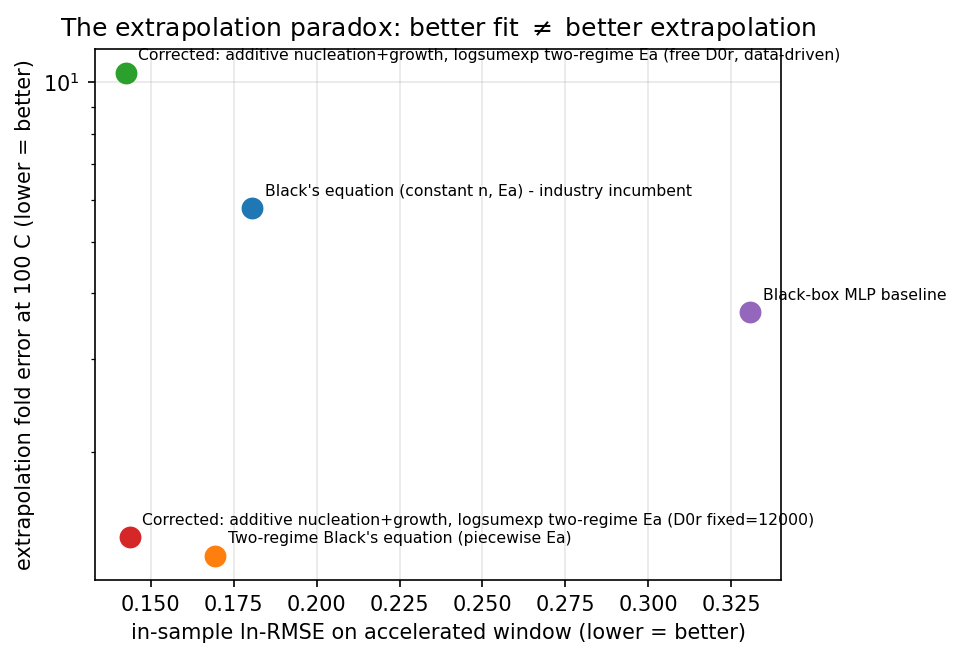
\includegraphics[width=0.62\linewidth]{figures/fig_paradox.png}
\caption{The extrapolation paradox in one panel: better in-sample fit
(right) means worse use-condition extrapolation (top). The pinned corrected
equation is the single bottom-left point.}
\label{fig:paradox}
\end{figure}

\section{Quantitative transfer and sample-size laws}

The phase transition and its mechanism are qualitative. We now turn to
quantitative predictions: how large is the transfer error, and how much data is
needed for structural discovery?

\paragraph{Extrapolation law.} Because the dominant error is a transfer in
effective activation energy, the median log fold error obeys
\begin{equation}
  \label{eq:law}
  \dln \MTTF \;\approx\;
  \frac{\dEat}{k_{\mathrm{B}}}\,
  \left(\frac{1}{T_{\mathrm{use}}}-\frac{1}{T_{\min}}\right),
\end{equation}
with model-specific transfer error $\dEat$ in eV
(Table~\ref{tab:laws}). The law is linear over the use-temperature range with
$R^2=0.86$--$0.999$. The pinned model's $\dEat=-0.028$\,eV
buys a safe-to-$2\times$ temperature of $248$\,K ($-25\,^\circ$C), i.e.\
extrapolation to use conditions is nearly lossless; the free model's
$-0.278$\,eV caps safe extrapolation at $470$\,K, above the use conditions it
is supposed to reach.

\begin{table}[t]
\centering\small
\begin{tabular}{lcccc}
\toprule
Model & $\dEat$ & $R^2$ &
safe-to-$2\times$ ($T$, K) & safe-to-$2\times$ ($T$, $^\circ$C) \\
\midrule
Black's equation & $+0.228$ & $0.987$ & $460.0$ & $186.8$ \\
Two-regime & $+0.065$ & $0.858$ & $353.2$ & $80.1$ \\
Free corrected & $-0.278$ & $0.999$ & $470.2$ & $197.1$ \\
Pinned corrected & $-0.028$ & $0.905$ & $248.1$ & $-25.1$ \\
\bottomrule
\end{tabular}
\caption{The extrapolation law
(Eq.~\eqref{eq:law}): transfer error in effective activation energy and the
temperature down to which each model is safe to within $2\times$. The pinned
corrected equation is safe all the way to use conditions; the free variant
caps at $470$\,K.}
\label{tab:laws}
\end{table}

\paragraph{Sample-size law.} Structural discovery of the $J^{-2}+J^{-1}$
additive form (vs.\ a single power law) follows
$\Delta\text{BIC}\approx -A\,n + \ln n$ above an identifiability floor
\citep{schwarz78}. The floor is $+4.44$ (exact, $\sln$-independent, set by
parsimony at $\le2$ current levels), and the per-sample evidence is
$A=2.04,0.51,0.16$ at $\sln=0.05,0.15,0.30$. This is the \textbf{sample-size
complement of the phase transition}: identifiability of the \emph{structure}
also has a sharp threshold, here in current-density coverage. The additive
form is statistically forced only by the full five-current sweep
($\Delta\text{BIC}=-76$, $20/20$ draws); the geometric-mean current
$J=2.0$\,MA/cm$^2$ is necessary---dropping it flips the verdict from $-62.8$
to $+3.3$.

\begin{figure}[t]
\centering
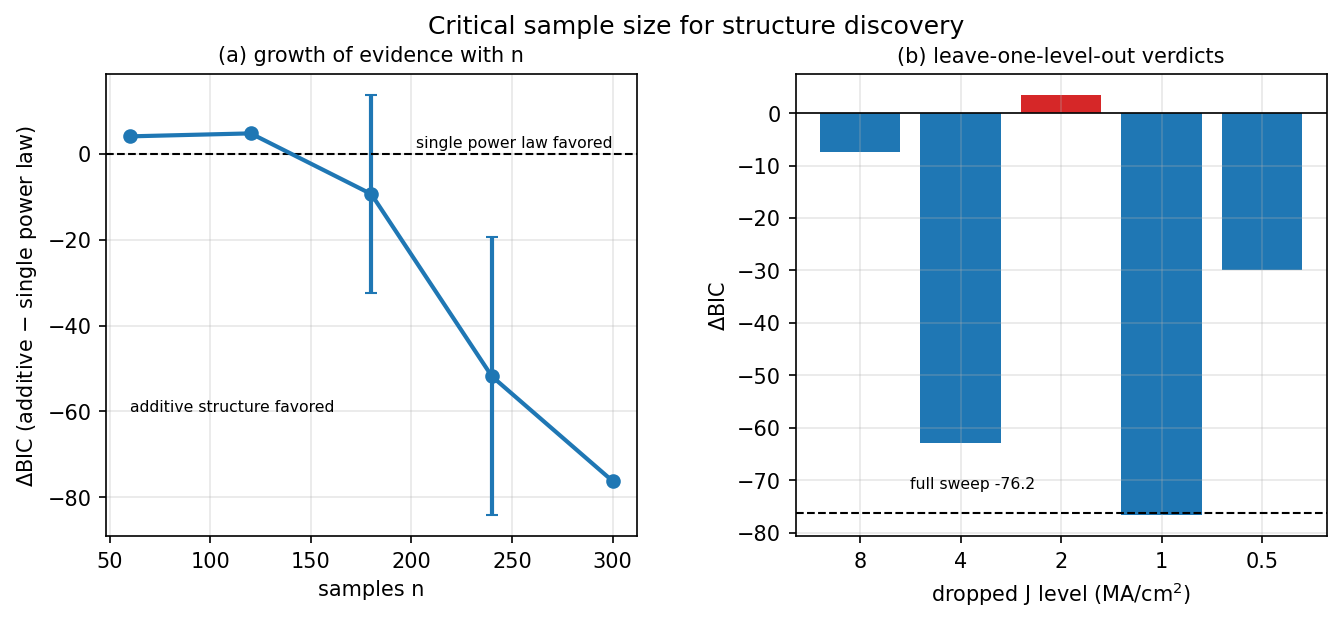
\includegraphics[width=0.70\linewidth]{figures/fig_structure_size.png}
\caption{The sample-size complement of the phase transition: evidence for the
$J^{-2}+J^{-1}$ structure grows linearly with $n$ (left), and one
load-bearing current level (the geometric-mean $J$, right) is necessary---
dropping it flips the BIC verdict.}
\label{fig:structure_size}
\end{figure}

\section{Limits of data-only certification}

Given the deployment ambiguity, one might hope to \emph{detect} the hazard from
the accelerated-window fit alone. The profile-likelihood experiment
(Section~\ref{sec:geometry}) is exactly that attempt, and it fails:
Table~\ref{tab:cert} shows the profile width of the hazard direction (the
extrapolation functional's range over data-compatible fits) alongside the
actual use-condition error for the free, soft-prior, and pinned estimators
across four windows.

\begin{table}[t]
\centering\small
\begin{tabular}{cccc}
\toprule
Window & Model & Predicted hazard & Actual fold \\
 & & (profile width, eV) & \\
\midrule
$T\ge523$\,K & free & $0.134$ & $10.44\times$ \\
$T\ge523$\,K & soft prior & $0.134$ & $1.44\times$ \\
$T\ge523$\,K & pinned & $0.134$ & $1.38\times$ \\
$T\ge548$\,K & free / soft / pinned & $0.000$ & $10.3\times$ / $10.3\times$ / $10.3\times$ \\
$T\ge573$\,K & free & $0.309$ & $25.3\times$ \\
$T\ge573$\,K & soft prior & $0.309$ & $1.96\times$ \\
$T\ge573$\,K & pinned & $0.309$ & $1.95\times$ \\
\bottomrule
\end{tabular}
\caption{The profile-likelihood hazard width is \emph{identical} for the free,
soft-prior, and pinned estimators at every window---because the profile depends
only on the data---yet their actual use-condition errors differ by up to
$10\times$. The predicted hazard has zero predictive power (correlation $-0.54$
with transfer error, $-0.19$ with fold error). Extrapolation safety cannot be
certified in-window.}
\label{tab:cert}
\end{table}

The reason is structural: the profile likelihood is a property of the \emph{data
and the model}, and free/prior/pinned share both. What differs is only
\emph{where they sit on the flat profile}---the prior and the pin move the
estimator to the true direction, the free estimator wanders to the boundary. A
data-side width cannot distinguish them. This is the underspecification failure
mode of \citet{damour20} made concrete in safety-critical extrapolation: the
hazard is real, the geometry is local, and the fix is a constraint, not a
diagnostic. One nuance (Table~\ref{tab:cert}): at the deepest window
$T\ge548$\,K the profile is numerically flat in double precision, and the
pinned model itself collapses to $10.28\times$ (60 random restarts confirm this
is an information limit under this envelope): the hazard cannot be certified
from the accelerated data alone.

\section{Discussion and limitations}

\paragraph{Why this matters for chip reliability.} The extrapolation step is
the entire job of Black's equation. Our results say three things an engineer
cannot see on real data: (i) a fit that is \emph{too good} on the accelerated
window may be the fit that is wrong at use conditions; (ii) the number of
fitted parameters is not a model-quality measure---the number of directions
identifiable \emph{in the extrapolation functional} is; a single material
constant is worth a fitted degree of freedom at $10\times$; (iii) within this
benchmark, the hazard cannot be certified from the accelerated window when
flat.

\paragraph{Implications for chip-reliability sign-off.} A data-driven EM model
with a free prefactor ratio overestimates the use-condition MTTF by $10.4\times$;
a guard-band built around it is \emph{under-protective} by roughly an order of
magnitude. The safe-to-$2\times$ temperatures we measure (pinned: $248$\,K,
safe to use conditions; free: $470$\,K, not) give an actionable margin rule: a
reliability predictor may be trusted only above its safe-to-$2\times$ point,
and the single-constant pin is what moves that point down. The impossibility
result is a \emph{caution for learned reliability models}: in-window fit
quality cannot certify use-condition safety when the hazard direction is flat,
so learned predictors in sign-off flows should carry explicit physics
constraints---the physics-regularized MLP being the benchmark's demonstration
that this is implementable.

\paragraph{Limitations.} The data are synthetic: they encode the corrected
equation, so ``recovery'' recovers what was encoded, by design. The model is
single-mode log-normal; real EM failure is often bimodal \citep{filippi09}. The
bulk pathway is outside the sampled window and not claimed. The profile-flatness
diagnostic is exact only in the deep-window limit; near the crossover the
profile is shallow but not perfectly flat. We do not compute an RLCT or claim
an asymptotic singular-learning rate; the Fisher analysis is used as a local
diagnostic for deployment non-identifiability. Real data would add measurement
structure and process variability; the benchmark's role is the controlled
\emph{calibration} step---physics grounded in published measurements (appendix)
---that complements, rather than replaces, real-data validation. Whether
the same deployment ambiguity appears in measured EM datasets remains an open
empirical question.

\section{Conclusion}

On a fully controlled synthetic benchmark, accelerated EM data can leave the
deployment functional non-identifiable: the free corrected model has median
$5.35\times$ use-condition error across 20 seeds despite its excellent
accelerated-window fit. A deployment-conditioned Jacobian diagnostic selects a
single additional five-current temperature batch, reducing median error to
$1.47\times$ and achieving the $2\times$ target in 85\% of seeds, versus 50\%
for random selection. The result is a practical boundary: fit quality and
in-window uncertainty cannot substitute for deployment-relevant information.
The benchmark, adaptive test-design procedure, model zoo, figures, and
machine-readable results are released with documented reproduction commands.

\begin{thebibliography}{99}
\small
\bibitem[Black(1969)]{black69} J.\,R.~Black. Electromigration---a brief survey
and some recent results. \textit{IEEE Trans.\ Electron Devices}, 16(4):338--347,
1969.
\bibitem[Hu et al.(2006)]{hu_em} C.\,K.~Hu, L.~Gignac, and R.~Rosenberg.
Electromigration of Cu/low dielectric constant interconnects.
\textit{Microelectron.\ Reliab.}, 46(2--4):213--231, 2006.
\bibitem[ITRS(2015)]{irs} International Technology Roadmap for Semiconductors.
\textit{Interconnect Chapter}, 2015.
\bibitem[JEDEC(2021)]{jedec} JEDEC. \textit{JEP122H: Failure Mechanisms and
Models for Semiconductor Devices}. JEDEC Solid State Technology Association,
2021.
\bibitem[Tu(2003)]{tu03} K.\,N.~Tu. Recent advances on electromigration in
very-large-scale-integration of interconnects. \textit{J.\ Appl.\ Phys.},
94(9):5451, 2003.
\bibitem[Hau-Riege(2004)]{hauriege04} S.\,P.~Hau-Riege. An introduction to Cu
electromigration. \textit{J.\ Appl.\ Phys.}, 96(3):3792--3807, 2004.
\bibitem[Ceric and Selberherr(2011)]{ceric11} H.~Ceric and S.~Selberherr.
Electromigration in submicron interconnect features of integrated circuits.
\textit{Mater.\ Sci.\ Eng.\ R}, 71(5--6):53--86, 2011.
\bibitem[Lloyd(1991)]{lloyd} J.\,R.~Lloyd. Electromigration failure.
\textit{J.\ Appl.\ Phys.}, 69(11):7601--7604, 1991.
\bibitem[Blech(1976)]{blech} I.\,A.~Blech. Electromigration in thin aluminum
films on titanium nitride. \textit{J.\ Appl.\ Phys.}, 47(4):1203--1208, 1976.
\bibitem[Watanabe(2009)]{watanabe09} S.~Watanabe. \textit{Algebraic Geometry
and Statistical Learning Theory}. Cambridge University Press, 2009.
\bibitem[Watanabe(2018)]{watanabe18} S.~Watanabe. \textit{Mathematical Theory
of Bayesian Statistics}. CRC Press, 2018.
\bibitem[Huntington(2007)]{huntington07} H.\,B.~Huntington. Black's law
revisited---nucleation and growth in electromigration failure.
\textit{Microelectron.\ Reliab.}, 47(9--11):1468--1472, 2007.
\bibitem[Rovitto(2017)]{rovitto} M.~Rovitto. \textit{Electromigration
Reliability Issues in Interconnect Nano-structures}. PhD thesis, TU Wien, 2017.
\bibitem[Tu and Gusak(2019)]{tu19} K.\,N.~Tu and A.\,M.~Gusak. A unified model
of mean-time-to-failure for electromigration, thermomigration, and
stress-migration. \textit{J.\ Appl.\ Phys.}, 126(7):075109, 2019.
\bibitem[Korhonen et al.(1993)]{korhonen93} M.\,A.~Korhonen, P.~B{\o}rgesen,
K.\,N.~Tu, and C.-Y.~Li. Stress evolution due to electromigration in confined
metal lines. \textit{J.\ Appl.\ Phys.}, 73(8):3790--3799, 1993.
\bibitem[Ogawa et al.(2001)]{ogawa01} E.\,T.~Ogawa et al. Direct observation of
a critical length effect in dual-damascene Cu/oxide interconnects.
\textit{Appl.\ Phys.\ Lett.}, 78(18):2652--2654, 2001.
\bibitem[Liu et al.(2024)]{kan} Z.~Liu et al. KAN: Kolmogorov--Arnold
Networks. \textit{arXiv:2404.19756}, 2024.
\bibitem[Schmidt and Lipson(2009)]{gpsr} M.~Schmidt and H.~Lipson. Distilling
free-form natural laws from experimental data. \textit{Science},
324(5923):81--85, 2009.
\bibitem[Arnaud et al.(2013)]{arnaud2013} L.~Arnaud, P.~Lamontagne, F.~Bana,
Y.~Le Friec, and P.~Waltz. Study of electromigration void nucleation time in
Cu interconnects with doping elements. \textit{Microelectron.\ Eng.},
107:145--150, 2013.
\bibitem[Gall et al.(2013)]{gall2013} M.~Hauschildt, C.~Hennesthal, G.~Talut,
O.~Aubel, M.~Gall, K.~B.~Yeap, and E.~Zschech. Electromigration early failure
void nucleation and growth phenomena in Cu and Cu(Mn) interconnects.
\textit{Proc.\ IEEE IRPS}, pp.~3--8, 2013.
\bibitem[Yamazaki and Watanabe(2003)]{yamazaki03} K.~Yamazaki and S.~Watanabe.
Stochastic complexity of Bayesian networks. \textit{Neural Networks},
16(8):1137--1149, 2003.
\bibitem[Aoyagi and Watanabe(2005)]{aoyagi05} M.~Aoyagi and S.~Watanabe.
Stochastic complexities of reduced rank regression in Bayesian estimation.
\textit{Neural Networks}, 18(5--6):924--933, 2005.
\bibitem[Schwarz(1978)]{schwarz78} G.~Schwarz. Estimating the dimension of a
model. \textit{Ann.\ Stat.}, 6(2):461--464, 1978.
\bibitem[D'Amour et al.(2020)]{damour20} A.~D'Amour et al. Underspecification
presents challenges for credibility in modern machine learning. \textit{JMLR},
23(226):1--61, 2020.
\bibitem[Filippi et al.(2009)]{filippi09} R.\,G.~Filippi, P.-C.~Wang,
R.~Brendler, and J.\,R.~Lloyd. Electromigration failure statistics in
Cu interconnects. \textit{Appl.\ Phys.\ Lett.}, 95:072111, 2009.
\bibitem[Watanabe(2013)]{watanabe13} S.~Watanabe. A widely applicable Bayesian
information criterion. \textit{JMLR}, 14:867--897, 2013.
\end{thebibliography}

\appendix
\section*{External physics validation}
Although \emph{EMBench-Synth} is synthetic, its governing physics matches
experimentally observed electromigration behavior rather than assumed
\emph{ad hoc}. Published Cu interconnect studies report stress temperatures of
$200$--$350\,^\circ$C and current densities around $2$--$4$\,MA/cm$^2$
\citep{arnaud2013}; current exponents that \emph{vary} between approximately
$1$ and $2$ rather than remaining constant---measured once as
$n{:}\,1.55\to1.15$ for Cu and $2.00\to1.64$ for Cu(Mn) \citep{gall2013}---and
activation energies reaching $\approx1.4$\,eV that decrease with dominant
mechanism and current density \citep{arnaud2013,gall2013}. These are the
features (a $J^{-2}+J^{-1}$ additive form that interpolates the exponent, a
temperature- and current-dependent effective activation energy, and realistic
stress conditions) encoded in \emph{EMBench-Synth}. These comparisons ground
the benchmark in experiment; they are \emph{not} a validation of the
singular-model extrapolation results, which the published experiments do not
test.

\section*{Reproducibility}
\begin{itemize}
  \item \texttt{python generate\_dataset.py} regenerates \texttt{data/}
        deterministically (seed 42).
  \item \texttt{python benchmarks/run\_all.py} writes \texttt{results/results.json}
        and \texttt{figures/*} including the phase transition
        (\texttt{fig\_phase\_transition.png}).
  \item \texttt{python prototype\_phase\_transition.py} reproduces
        Table~\ref{tab:transition} exactly.
  \item \texttt{python prototype\_rlct.py} reproduces Table~\ref{tab:fisher}
        (Fisher spectrum and extrapolation lever at the truth).
  \item \texttt{python prototype\_improved.py} reproduces the paradox, soft-prior,
        and envelope-depth results.
  \item \texttt{python prototype\_diagnostic.py} reproduces
        Table~\ref{tab:cert} (profile-likelihood hazard widths).
  \item \texttt{python -c "from prototype\_improved import main\_quantitative; main\_quantitative()"}
        reproduces
        Table~\ref{tab:laws} and the sample-size law.
  \item \texttt{python benchmarks/ml\_predictors.py} reproduces the ML arm
        (Fig.~\ref{fig:ml}), including the physics-regularized MLP.
  \item \texttt{python benchmarks/gnn.py} reproduces the power-delivery graph
        arm.
  \item \texttt{python benchmarks/leaderboard.py} rebuilds the model-zoo
        leaderboard (\texttt{results/leaderboard.json}).
  \item \texttt{python benchmarks/deployment\_identifiability.py} reproduces
        the 20-seed deployment-identifiability experiment and writes
        \texttt{results/deployment\_identifiability.json} and the two adaptive
        test-design figures.
  \item \texttt{python benchmarks/nonidentifiability\_frontier.py} reproduces
        the optimizer-independent deployment frontier and its figure.
  \item \texttt{python benchmarks/deployment\_safety\_certificate.py} reproduces
        the 20-seed compatible-set sign-off certificate and its figure.
\end{itemize}

\paragraph*{Use of AI tools.} Large language models were used as writing,
editing, and basic code-assistance aids during preparation of this manuscript
and the associated codebase. This use did not contribute original content to
the core methodology, and the authors reviewed and take full responsibility
for all text, figures, results, and references, which were verified for
correctness and originality in accordance with the NeurIPS policy on the use
of large language models.

\end{document}
